\begin{center}
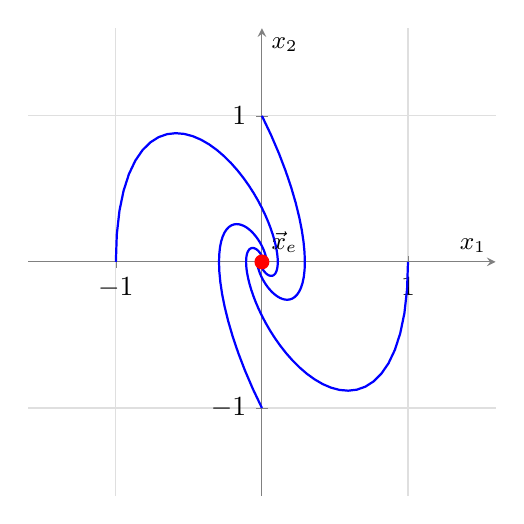
\begin{tikzpicture}
\begin{axis}[
  width=0.62\linewidth, height=0.62\linewidth,
  xlabel={$x_1$}, ylabel={$x_2$},
  axis lines=center,
  axis line style={gray},
  label style={font=\small},
  xmin=-1.6, xmax=1.6, ymin=-1.6, ymax=1.6,
  xtick={-1,0,1}, ytick={-1,0,1},
  grid=major, grid style={gray!25},
]
\addplot[domain=0:8, samples=120, thick, blue]
  ({exp(-x)*(cos(deg(sqrt(2)*x)) + (1/sqrt(2))*sin(deg(sqrt(2)*x)))},
   {-(3/sqrt(2))*exp(-x)*sin(deg(sqrt(2)*x))});
\addplot[domain=0:8, samples=120, thick, blue]
  ({(1/sqrt(2))*exp(-x)*sin(deg(sqrt(2)*x))},
   {exp(-x)*(cos(deg(sqrt(2)*x)) - (1/sqrt(2))*sin(deg(sqrt(2)*x)))});
\addplot[domain=0:8, samples=120, thick, blue]
  ({-exp(-x)*(cos(deg(sqrt(2)*x)) + (1/sqrt(2))*sin(deg(sqrt(2)*x)))},
   {(3/sqrt(2))*exp(-x)*sin(deg(sqrt(2)*x))});
\addplot[domain=0:8, samples=120, thick, blue]
  ({-(1/sqrt(2))*exp(-x)*sin(deg(sqrt(2)*x))},
   {-exp(-x)*(cos(deg(sqrt(2)*x)) - (1/sqrt(2))*sin(deg(sqrt(2)*x)))});
\addplot[only marks, mark=*, mark size=2.5pt, red] coordinates {(0,0)};
\node[above right, font=\small] at (axis cs:0,0) {$\vec{x}_e$};
\end{axis}
\end{tikzpicture}
\end{center}
